\documentclass[11pt]{article}
\usepackage[letterpaper, margin=1in]{geometry}
\usepackage[utf8]{inputenc}
\usepackage{graphicx}
\usepackage{float}
\usepackage{hyperref}
\usepackage{microtype}

\title{Design, Implementation, and Testing of a Pipelined Reliable Transfer Protocol}
\author{Neel Sadafule and Dylan Cantafio}
\date{December 2, 2024}

\begin{document}

\maketitle

\section{Introduction}

In this project, we designed and implemented a reliable data transfer protocol over UDP sockets in Python. The protocol incorporates flow control and congestion control mechanisms to ensure efficient and reliable communication over an unreliable network. Additionally, we simulated packet loss and corruption to test the robustness of our protocol under adverse network conditions.

\section{Protocol Design and Implementation}

\subsection{Overview}

Our protocol aims to provide reliable, connection-oriented communication on top of UDP, which is inherently unreliable and connectionless. To achieve this, we implemented features commonly found in TCP, such as sequence numbering, acknowledgments, checksums for error detection, flow control using a sliding window, and congestion control mechanisms.

\subsection{Packet Structure}

Each packet in our protocol consists of:

\begin{itemize}
    \item \textbf{Packet Type (1 byte):} Indicates the type of packet:
    \begin{itemize}
        \item \texttt{DATA} (0)
        \item \texttt{SYN} (1)
        \item \texttt{ACK} (2)
        \item \texttt{FIN} (3)
    \end{itemize}
    \item \textbf{Sequence Number (4 bytes):} A 32-bit number used to order packets.
    \item \textbf{Checksum (2 bytes):} A 16-bit checksum for error detection.
    \item \textbf{Payload (variable length):} The actual data being transmitted.
\end{itemize}

\subsection{Connection Management}

\subsubsection{Connection Establishment}

We implemented a three-way handshake to establish a connection:

\begin{enumerate}
    \item \textbf{SYN:} The sender initiates the connection by sending a \texttt{SYN} packet with sequence number 0.
    \item \textbf{SYN-ACK:} The receiver responds with a \texttt{SYN} packet (serving as \texttt{SYN-ACK}).
    \item \textbf{ACK:} The sender sends an \texttt{ACK} packet to complete the handshake.
\end{enumerate}

\subsubsection{Connection Termination}

Connection termination is handled using a two-way handshake:

\begin{enumerate}
    \item \textbf{FIN:} The sender sends a \texttt{FIN} packet to initiate termination.
    \item \textbf{FIN-ACK:} The receiver responds with a \texttt{FIN} packet (\texttt{FIN-ACK}).
\end{enumerate}

\subsection{Reliability Mechanisms}

\subsubsection{Sequence Numbers and Acknowledgments}

\begin{itemize}
    \item \textbf{Sequence Numbers:} Each data packet is assigned a unique sequence number to ensure proper ordering.
    \item \textbf{Acknowledgments:} The receiver sends \texttt{ACK} packets with the sequence number of the received packet to confirm successful reception.
\end{itemize}

\subsubsection{Checksums for Error Detection}

We compute a checksum by summing the packet type, sequence number, and payload bytes. The receiver recalculates the checksum upon receiving a packet to detect any corruption.

\subsubsection{Timeouts and Retransmissions}

\begin{itemize}
    \item The sender starts a timer for each packet sent.
    \item If an acknowledgment is not received within a specified timeout interval, the packet is retransmitted.
\end{itemize}

\subsection{Flow Control}

We implemented flow control using a sliding window protocol:

\begin{itemize}
    \item The sender maintains a window of unacknowledged packets.
    \item The window size is controlled by the congestion window (\texttt{cwnd}), ensuring the sender does not overwhelm the receiver.
    \item Multiple in-flight packets are allowed within the sliding window, ensuring efficient utilization of the network while maintaining reliability. Once an acknowledgment (\texttt{ACK}) is received, the window slides forward to include new packets.
\end{itemize}

\subsection{Congestion Control}

Our congestion control mechanism is inspired by TCP's slow start and congestion avoidance phases. The congestion window (\texttt{cwnd}) is dynamically adjusted based on network conditions to balance efficient data transfer and avoid congestion.

\begin{itemize}
    \item \textbf{Slow Start Phase:} During the slow start phase, the \texttt{cwnd} increases exponentially as packets are successfully acknowledged by the receiver.
    \item \textbf{Congestion Avoidance Phase:} Once \texttt{cwnd} exceeds the slow start threshold (\texttt{ssthresh}), the protocol transitions to congestion avoidance. Here, \texttt{cwnd} increases linearly, ensuring network stability and avoiding excessive traffic.
    \item \textbf{Packet Loss Handling:} When packet loss is detected (e.g., through a timeout or duplicate ACKs), \texttt{ssthresh} is set to half of the current \texttt{cwnd}, and \texttt{cwnd} is reset to 1. This ensures a gradual recovery while minimizing the risk of further congestion.
\end{itemize}

\subsection{Simulation of Packet Loss and Corruption}

To test the protocol under adverse conditions, we simulated packet loss and corruption:

\begin{itemize}
    \item \textbf{Packet Loss:} Implemented by randomly dropping packets with a certain probability (\texttt{LOSS\_PROBABILITY}).
    \item \textbf{Packet Corruption:} Simulated by randomly altering packets with a certain probability (\texttt{ERROR\_PROBABILITY}). Corrupted packets are detected using checksums and discarded by the receiver.
\end{itemize}

\section{Testing and Results}

\subsection{Testing Environment}

\begin{itemize}
    \item \textbf{Hardware and Software:}
    \begin{itemize}
        \item MacBook Pro running macOS.
        \item Python 3.x for both \texttt{sender.py} and \texttt{receiver.py}.
    \end{itemize}
    \item \textbf{Testing Tools:}
    \begin{itemize}
        \item Wireshark for capturing and analyzing network traffic.
        \item \texttt{tcpdump} for capturing packets on the loopback interface. (\texttt{sudo tcpdump -i lo0 -w lo0\_capture.pcap})
        \item \texttt{wget} execute a large file download.
        (\texttt{wget http://speedtest.tele2.net/10MB.zip})
    \end{itemize}
\end{itemize}

\subsection{Test Procedures}

We conducted tests to verify the correctness and performance of our protocol under various network conditions.

\begin{enumerate}
    \item \textbf{Baseline Test:}
    \begin{itemize}
        \item Set \texttt{LOSS\_PROBABILITY} and \texttt{ERROR\_PROBABILITY} to 0.
        \item Verified that data transfer occurs correctly without any loss or corruption.
    \end{itemize}
    \item \textbf{Packet Loss Simulation:}
    \begin{itemize}
        \item Set \texttt{LOSS\_PROBABILITY} to 0.1.
        \item Observed the sender retransmitting packets upon timeouts.
        \item Verified that all data packets were eventually received and acknowledged.
    \end{itemize}
    \item \textbf{Packet Corruption Simulation:}
    \begin{itemize}
        \item Set \texttt{ERROR\_PROBABILITY} to 0.05.
        \item Observed the receiver detecting corrupted packets and discarding them.
        \item Verified that the sender retransmitted the corrupted packets after timeouts.
    \end{itemize}
    \item \textbf{Combined Loss and Corruption:}
    \begin{itemize}
        \item Tested with both \texttt{LOSS\_PROBABILITY} and \texttt{ERROR\_PROBABILITY} set to non-zero values.
        \item Ensured the protocol handled both lost and corrupted packets effectively.
    \end{itemize}
\end{enumerate}

\subsection{Results and Analysis}

\subsubsection{Connection Establishment and Termination}

The three-way handshake successfully established a connection before data transfer, and connection termination was handled gracefully after all data was transmitted.

\begin{figure}[H]
    \centering
     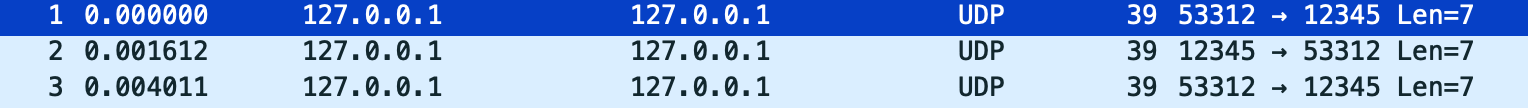
\includegraphics[width=0.8\textwidth]{handshake_capture.png}
    \caption{Wireshark Capture of the Three-Way Handshake. The capture highlights the SYN, SYN-ACK, and ACK packets exchanged between the sender (port 53312) and the receiver (port 12345).}
    \label{fig:handshake}
\end{figure}

\begin{figure}[H]
    \centering
     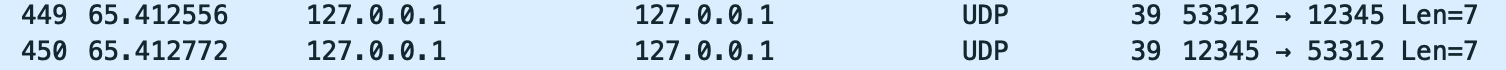
\includegraphics[width=0.8\textwidth]{termination_capture.png}
    \caption{Wireshark Capture of the Connection Termination. The capture shows the FIN packet sent by the sender and the FIN-ACK packet sent by the receiver to gracefully terminate the connection.}
    \label{fig:termination}
\end{figure}

\subsubsection{Data Transfer and Reliability}

The sender adjusted the congestion window (\texttt{cwnd}) based on network conditions. The sliding window mechanism effectively managed flow control, and all data segments were eventually received in order, demonstrating reliability.

\begin{figure}[H]
    \centering
    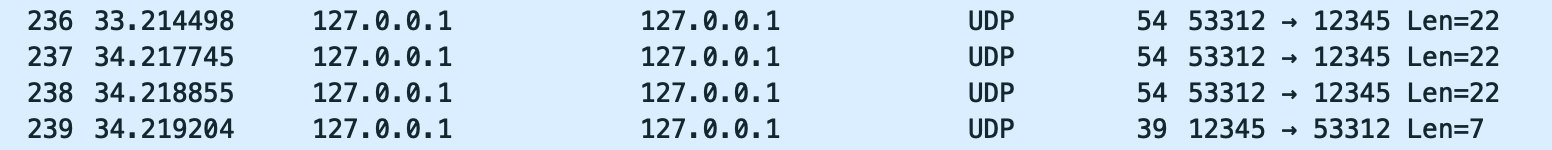
\includegraphics[width=0.8\textwidth]{sliding_window_capture.png}
    \caption{Illustration of the Sliding Window Protocol in Operation. Packets 236, 237, and 238 represent in-flight packets sent consecutively without waiting for acknowledgments. Packet 239 is an acknowledgment sent from the receiver confirming successful reception of earlier packets.}
    \label{fig:sliding_window_flow}
\end{figure}

\subsubsection{Congestion Control Behavior}

We observed the congestion window (\texttt{cwnd}) increasing exponentially during the slow start phase and linearly during the congestion avoidance phase. Upon detecting packet loss, \texttt{cwnd} was reduced, and the protocol re-entered slow start.

\begin{figure}[H]
    \centering
    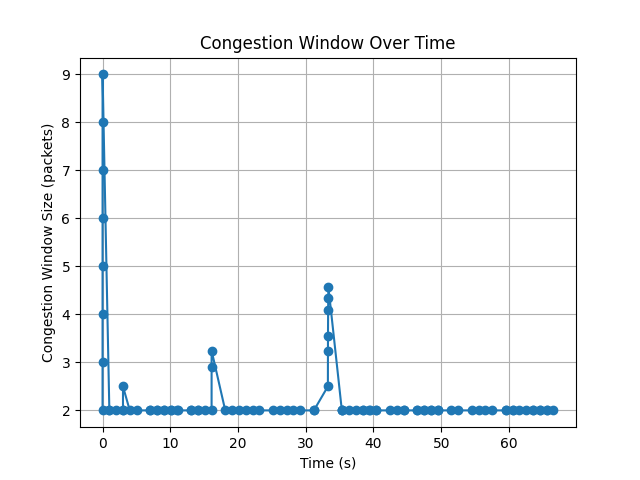
\includegraphics[width=0.8\textwidth]{cwnd_plot.png}
    \caption{Congestion Window (\texttt{cwnd}) Over Time. The graph highlights exponential growth during slow start and linear growth during congestion avoidance.}
    \label{fig:cwnd_plot}
\end{figure}


\begin{itemize}
    \item \textbf{Initial Growth:} The \texttt{cwnd} increases rapidly, demonstrating the slow start phase, where the congestion window grows exponentially until it reaches the slow start threshold (\texttt{ssthresh}).
    \item \textbf{Packet Loss Response:} After packet loss or congestion is detected (indicated by a timeout), the congestion window size drops sharply to its minimum and re-enters the slow start phase.
    \item \textbf{Periodic Spikes:} The periodic spikes in \texttt{cwnd} around 10 and 30 seconds reflect moments when the network briefly allows more packets before encountering congestion, at which point \texttt{cwnd} is reduced.
    \item \textbf{Stabilization:} Over time, \texttt{cwnd} stabilizes at lower levels, showing the protocol's adaptability to the network's capacity and its ability to prevent further congestion.
\end{itemize}

Additionally, we captured a screenshot of the congestion window behavior during slow start, highlighting the initial exponential growth:

\begin{figure}[H]
    \centering
    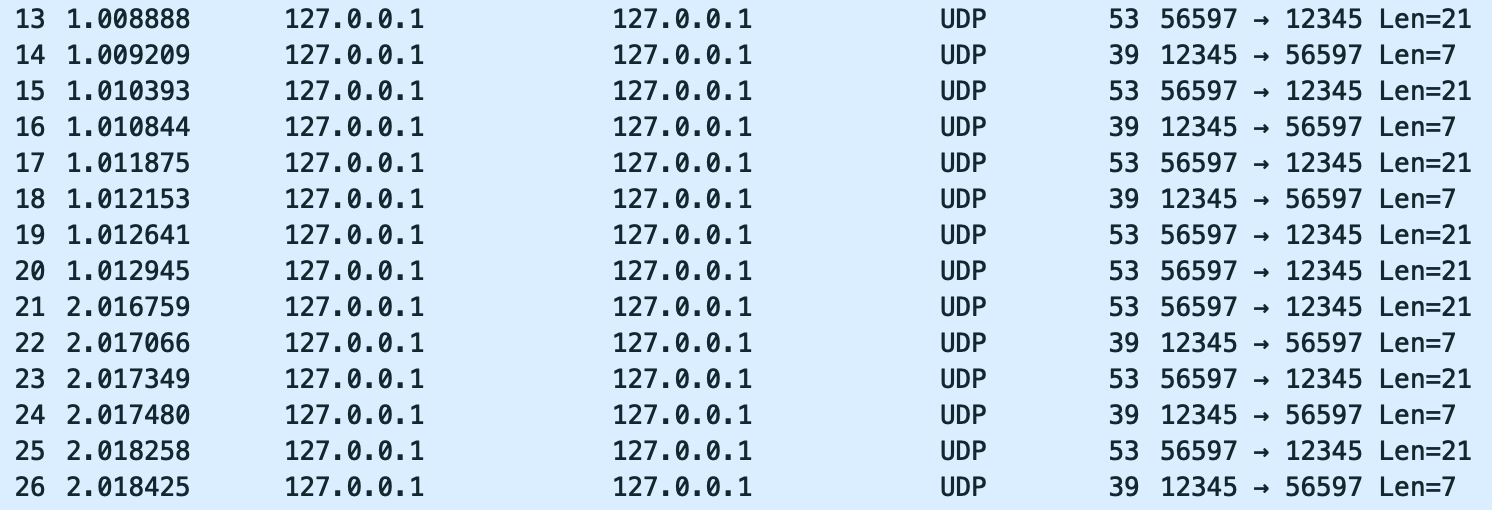
\includegraphics[width=0.8\textwidth]{screenshot_cwnd.png}
    \caption{Congestion Window (\texttt{cwnd}) During Slow Start. Packets 13–26 demonstrate exponential growth of \texttt{cwnd}, evidenced by the rapid transmission and minimal gaps in timestamps.}
    \label{fig:cwnd_slow_start}
\end{figure}

\subsubsection{Latency (Round-Trip Time - RTT)}

Latency, measured as the round-trip time (RTT) for each packet, was observed to increase during periods of congestion or retransmissions. Figure \ref{fig:latency_plot} shows RTT spikes corresponding to packet retransmissions and congestion events, reflecting the protocol's handling of adverse network conditions.

\begin{figure}[H]
    \centering
    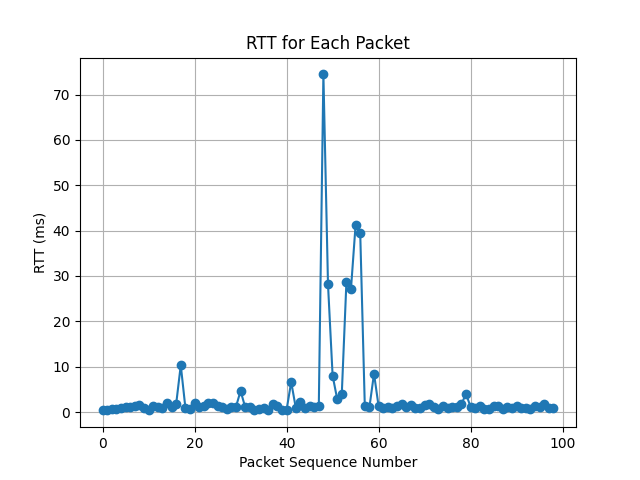
\includegraphics[width=0.8\textwidth]{latency_plot.png}
    \caption{RTT for Each Packet. Spikes indicate increased latency during packet retransmissions and congestion.}
    \label{fig:latency_plot}
\end{figure}

\begin{itemize}
    \item \textbf{Consistent RTTs:} For most packets, the RTT remains consistent and low, indicating smooth transmission conditions.
    \item \textbf{Spikes in RTT:} Spikes are observed for certain packets, especially around sequence numbers 40–60. These spikes likely correspond to:
    \begin{itemize}
        \item \textbf{Retransmissions:} Due to packet loss or corruption, additional time is required to send and acknowledge a packet.
        \item \textbf{Congestion:} Higher network congestion increases delays in receiving acknowledgments, leading to elevated RTT values.
    \end{itemize}
    \item \textbf{Stabilization After Spikes:} After the spikes, the RTT stabilizes, demonstrating that the protocol efficiently adapts to network conditions and mitigates the effects of congestion or packet loss.
\end{itemize}

\subsubsection{Throughput}

The throughput, measured in bits per second (bps), shows how efficiently the protocol utilized the available network capacity over time. As illustrated in Figure \ref{fig:throughput_plot}, throughput varies with network conditions.

\begin{figure}[H]
    \centering
    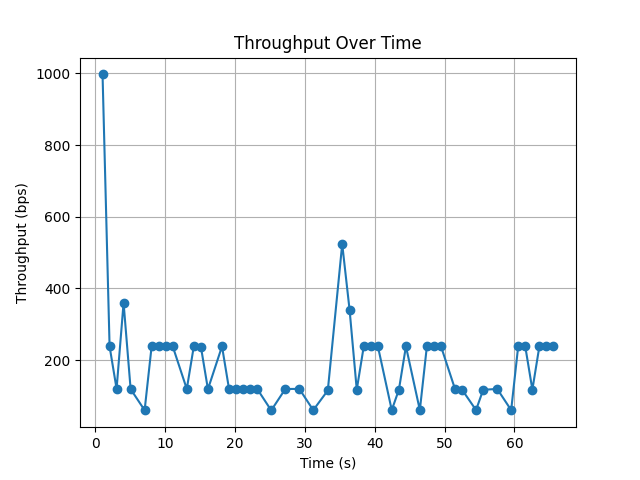
\includegraphics[width=0.8\textwidth]{throughput_plot.png}
    \caption{Throughput Over Time. The graph shows fluctuations caused by network conditions and retransmissions.}
    \label{fig:throughput_plot}
\end{figure}

\begin{itemize}
    \item \textbf{High Initial Throughput:} The initial throughput is very high, reflecting the rapid transmission of data during the early stages when \texttt{cwnd} is increasing.
    \item \textbf{Drops Due to Retransmissions:} The drops in throughput correspond to periods of packet loss or retransmissions, where effective transmission temporarily decreases as the protocol compensates for lost or corrupted packets.
    \item \textbf{Spikes Corresponding to \texttt{cwnd} Expansion:} Spikes in throughput, such as around 30 seconds, align with moments when the congestion window briefly expands, allowing more packets to be sent and acknowledged successfully.
    \item \textbf{Stabilization Over Time:} The overall trend shows a decrease in throughput over time as the protocol stabilizes in response to network conditions, maintaining reliable communication rather than maximizing speed.
\end{itemize}

\subsubsection{Handling of Packet Loss and Corruption}

The protocol successfully detected and handled packet loss through retransmissions. Packet corruption was detected using checksums, and corrupted packets were retransmitted.

\begin{figure}[H]
    \centering
    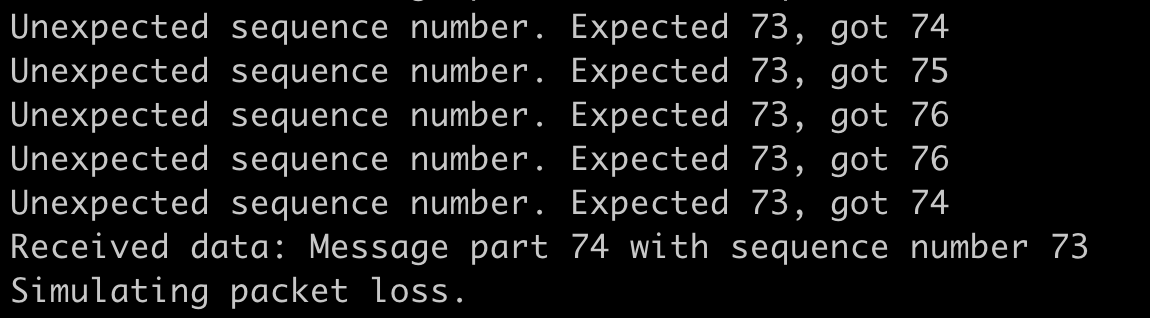
\includegraphics[width=0.8\textwidth]{packet_loss_receiver.png}
    \caption{Logs showing the receiver simulating packet loss for sequence number 73.}
    \label{fig:packet_loss_receiver}
\end{figure}
\begin{figure}[H]
    \centering
    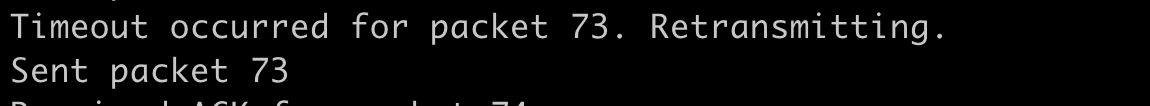
\includegraphics[width=0.8\textwidth]{packet_loss_sender.png}
    \caption{Logs showing the sender retransmitting packet 73 after a timeout.}
    \label{fig:packet_loss_sender}
\end{figure}

\begin{figure}[H]
    \centering
    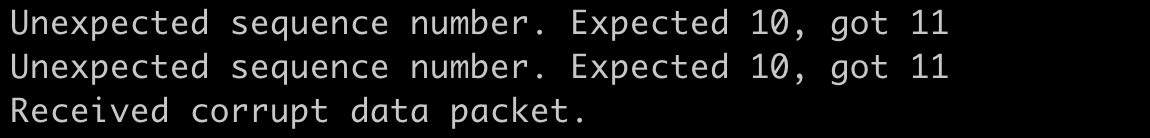
\includegraphics[width=0.8\textwidth]{packet_corruption_receiver.png}
    \caption{Logs showing the receiver discarding a corrupted packet with sequence number 10.}
    \label{fig:packet_corruption_receiver}
\end{figure}
\begin{figure}[H]
    \centering
    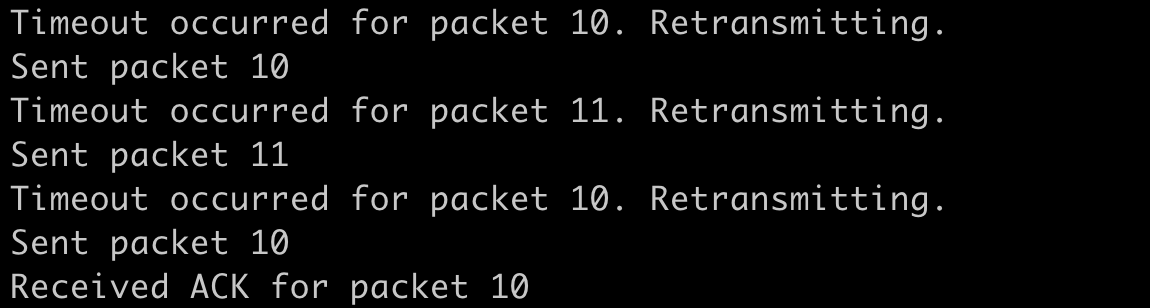
\includegraphics[width=0.8\textwidth]{packet_corruption_sender.png}
    \caption{Logs showing the sender retransmitting packet 10 after detecting corruption.}
    \label{fig:packet_corruption_sender}
\end{figure}

The results demonstrate that the protocol successfully handles both packet loss and corruption:

\begin{itemize}
    \item \textbf{Robustness to Packet Loss:} The sliding window mechanism ensures that lost packets are retransmitted, maintaining reliability.
    \item \textbf{Error Detection and Correction:} Checksums effectively detect corrupted packets, and retransmissions ensure data integrity.
    \item \textbf{Adaptation to Network Conditions:} The congestion control algorithm effectively adjusts the sending rate based on network feedback, balancing efficiency and fairness.
\end{itemize}

\subsection{Fairness and Coexistence}

To evaluate the fairness of our protocol, we conducted additional tests where it operated concurrently with standard TCP traffic generated by separate `wget` commands downloading the file from [Speedtest](http://speedtest.tele2.net/10MB.zip). This setup allowed us to observe how our protocol behaves under realistic network conditions with competing traffic.

\subsubsection{Congestion Window Over Time}

The plot \textbf{"Congestion Window Over Time"} (Figure \ref{fig:cwnd_fairness}) reflects the dynamic adjustments of the congestion window (\texttt{cwnd}) as the protocol interacts with both network conditions and competing TCP traffic from three `wget` commands.

\begin{figure}[H]
    \centering
    \includegraphics[width=0.8\textwidth]{cwnd_plot_fairness.png}
    \caption{Congestion Window (\texttt{cwnd}) Over Time with Concurrent TCP Traffic. The plot shows how \texttt{cwnd} adjusts in response to competing `wget` traffic, demonstrating fairness in bandwidth sharing.}
    \label{fig:cwnd_fairness}
\end{figure}

\begin{itemize}
    \item \textbf{Initial Behavior and Slow Start Phase:} At the beginning of the transfer, the congestion window increases exponentially during the slow start phase, peaking at approximately 5.5 packets. This phase occurs before any significant network contention from the first `wget` command, allowing the protocol to probe the network's available bandwidth effectively.
    
    \item \textbf{Impact of the First wget Command:} Around the 5-second mark, the congestion window begins to drop sharply. This corresponds to the first `wget` download introducing TCP traffic into the network. The congestion window stabilizes between 2 and 4 packets, indicating that the protocol has detected increased network congestion and transitioned to the congestion avoidance phase.
    
    \item \textbf{Subsequent TCP Traffic:} Each successive `wget` command causes similar drops in the congestion window, showcasing the protocol's responsiveness to bursts of competing traffic. Between these drops, the congestion window remains stable at a lower level, allowing fair coexistence with the TCP flows.
    
    \item \textbf{Recovery and Final Behavior:} After the last `wget` command completes, the congestion window increases again, peaking toward the end of the session. This recovery demonstrates the protocol’s ability to reclaim bandwidth when network conditions improve.
\end{itemize}

\subsubsection{Round-Trip Time (RTT) for Each Packet}

The plot \textbf{"RTT for Each Packet"} (Figure \ref{fig:latency_fairness}) illustrates the variations in Round-Trip Time (RTT) for packets during the session with concurrent TCP traffic.

\begin{figure}[H]
    \centering
    \includegraphics[width=0.8\textwidth]{latency_plot_fairness.png}
    \caption{RTT for Each Packet with Concurrent TCP Traffic. The plot shows RTT spikes corresponding to periods of high network contention due to `wget` downloads.}
    \label{fig:latency_fairness}
\end{figure}

\begin{itemize}
    \item \textbf{Baseline RTT:} During the initial phase of the transfer (before the first `wget` command), RTT values are consistently low, indicating minimal network congestion.
    
    \item \textbf{Increased RTT During TCP Traffic:} Each `wget` command introduces competing traffic, causing RTT spikes of up to 3 ms. These spikes align with the drops in the congestion window in the first plot, confirming that the additional TCP traffic increased network contention.
    
    \item \textbf{Stabilization After TCP Traffic:} Once the competing `wget` traffic subsides, RTT values stabilize, with minor fluctuations. This demonstrates that the protocol recovers well after periods of contention, maintaining low latency when the network load decreases.
\end{itemize}

\subsubsection{Throughput Over Time}

The plot \textbf{"Throughput Over Time"} (Figure \ref{fig:throughput_fairness}) highlights the protocol's ability to transfer data effectively while coexisting with competing TCP traffic.

\begin{figure}[H]
    \centering
    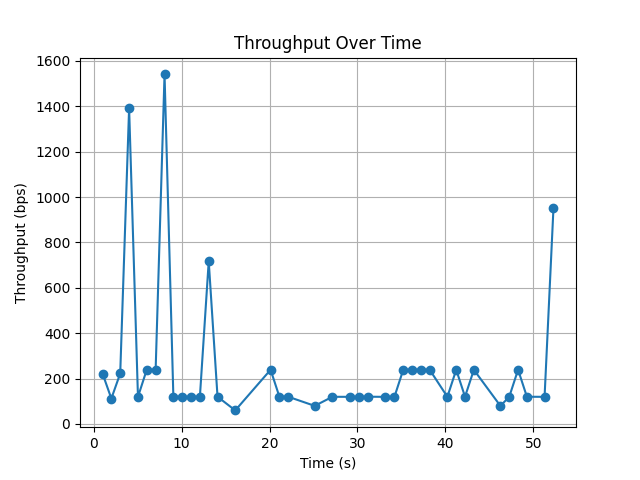
\includegraphics[width=0.8\textwidth]{throughput_plot_fairness.png}
    \caption{Throughput Over Time with Concurrent TCP Traffic. The plot shows how throughput fluctuates in response to competing `wget` traffic, reflecting the protocol's fair bandwidth sharing.}
    \label{fig:throughput_fairness}
\end{figure}

\begin{itemize}
    \item \textbf{Initial High Throughput:} At the start of the transfer, throughput peaks at around 1600 bps, corresponding to the slow start phase of the congestion window. This period occurs before any `wget` traffic is introduced, allowing the protocol to maximize its use of the network.
    
    \item \textbf{Impact of TCP Traffic:} Each `wget` command introduces significant reductions in throughput. These drops correspond to the congestion window decreases in the first plot, as the protocol reduces its sending rate to accommodate the competing TCP flows.
    
    \item \textbf{Recovery After Congestion:} Once the final `wget` download completes, the protocol’s throughput increases again, demonstrating its ability to recover bandwidth when the network contention decreases. The final peak in throughput aligns with the increase in the congestion window, indicating efficient utilization of available resources.
\end{itemize}

\section{Conclusion}

Our implementation of a pipelined reliable transfer protocol over UDP successfully achieved reliable, ordered, and efficient data transfer. The incorporation of flow control and congestion control mechanisms allowed the protocol to adapt to varying network conditions and maintain acceptable performance. Simulating packet loss and errors verified the robustness of the protocol, demonstrating its ability to handle adverse network scenarios.\\\\
Furthermore, we evaluated the fairness and coexistence capabilities of our protocol by running it concurrently with standard TCP traffic generated by separate \texttt{wget} commands downloading data from \url{http://speedtest.tele2.net/10MB.zip}. The results from the congestion window (\texttt{cwnd}), Round-Trip Time (RTT), and throughput plots indicate that our protocol reduces its sending rate during periods of high contention from the \texttt{wget} commands. This behavior demonstrates fairness by allowing the competing TCP flows to utilize the network without being starved of bandwidth.\\\\
The protocol's responsiveness to network conditions is evident from its dynamic adjustments to the congestion window, RTT stabilization, and throughput recovery in response to the introduction and completion of competing traffic. During periods of concurrent \texttt{wget} traffic, the protocol avoids monopolizing bandwidth and shares network resources effectively. Once the competing traffic subsides, it increases its sending rate to utilize the available bandwidth efficiently.\\\\
These results provide strong evidence that the protocol is fair and capable of coexisting with standard TCP traffic. The dynamic behavior observed in the plots aligns with the principles of congestion control and fairness, demonstrating that the protocol can adapt to network conditions and share resources equitably.\\\\
In summary, our protocol not only ensures reliable and efficient data transfer over an unreliable network but also maintains fairness and adaptability in the presence of competing network traffic. This dual capability underscores the protocol's robustness and suitability for diverse networking environments.

\end{document}
